Let $M=(x_0,y_0)$ be a fixed point. Referring to Equation~\ref{eqn:support}, the pedal of $M$ is given by

\begin{equation}\label{eq:pedal}
 P_M(t)= [  x_0 \sin^2 t + \left( h(t) -y_0\sin
 t    \right) \cos t, \left( h(t) -{  x_0}\,\cos t  
   \right) \sin t +   y_0\cos^2 t ].
\end{equation}


The contrapedal of $M$ (intersection of the line $M+s \mathcal{C}'(t)$ and the normal line $\mathcal{C}(s)+u\mathcal{C}'(t)^{\perp}$) is given by

\begin{equation}\label{eq:contrapedal}
C_M(t)=  [ x_0  \cos^2t   +y_0\cos t
 \sin t -h'(t) \sin t , y_0 \sin^2t
 +x_0\cos t \sin t 
	 + h'(t) \cos t]
.
\end{equation}

Below is a generalization of Corollary~\ref{cor:area-diff}.


\begin{proposition}
For all convex curves, the following holds:
	\[A(P_M)-A(C_M)=A(\mathcal{C})\]
	\label{prop:darea}

\end{proposition}

\begin{proof}
Obtain the signed areas for the above curves above via integration by parts of  Equation~\ref{eqn:area}. Algebraic manipulation yields the claim.
In fact, 
\begin{align*}
A(P_M)=& \frac{\pi}{2}(x_0^2+y_0^2)- \left(\int_0^{2\pi}\!\!\!\!\!\!h(t)\cos t dt\right) x_0- \left(\int_0^{2\pi}\!\!\!\!\!\!h(t)\sin t dt \right) y_0+\frac{1}{2}  \int_0^{2\pi}\!\!\!\!\!\!h(t)^2 dt\\
A(C_M)=& \frac{\pi}{2}(x_0^2+y_0^2)- \left(\int_0^{2\pi}\!\!\!\!\!\!{h(t)\cos{t}dt}\right) x_0- \left(\int_0^{2\pi}\!\!\!\!\!\!h(t)\sin t dt \right) y_0+\frac{1}{2}\int_0^{2\pi}\!\!\!\!\!\!h^\prime(t)^2 dt\\
A(\mathcal{C})=& \frac{1}{2}\int_0^{2\pi}\!\!\!\!\!(h(t)^2-h^{\prime}(t)^2)dt
%
\end{align*}
\end{proof}

%\begin{corollary}
%For any plane curve with vanishing signed area, $A(P_M)=A(C_M)$
%\end{corollary}

\begin{corollary} The family of isocurves of $A(P_M)$ and $A(C_M)$ are circles centered at
	
	\begin{align*}
	\label{eq:centroK}
K=\left(	\frac{1}{\pi} \int_0^{2\pi}\!\!\!\!\! h(t)\cos t \,dt,	\frac{1}{\pi} \int_0^{2\pi}\!\!\!\!\! h(t)\sin t \, dt\right)
	\end{align*}
	
	
\end{corollary}

\begin{proof} Direct from the definition of the centroid  $K=\frac{1}{2\pi}\int_0^{2\pi}\mathcal{C}(t)dt$ and expressions of the areas $A(P_M)$ and $A(C_M)$.
\end{proof}

\begin{proposition} Let $P_{ {\theta }M}$ the pedal of $M$ with respect to the curve $\mathcal{C}_\theta$.  For any convex curve $\mathcal{C}$ we have that:
	\[A(P_M)-A(P_{ {\theta }M})=\sin^2\theta A(\mathcal{C})\]
	
	\end{proposition}

\begin{proof} Similar to the that of Proposition \ref{prop:darea}.
\end{proof}

Referring to Figure~\ref{fig:interp-concave} and generalizing Proposition~\ref{prop:interpol}:

%\begin{proposition}
%\label{prop:amu}
%Let $\mathcal{C}_\mu=\mu P_M+(1-\mu)C_M$
	
%	Then, for $\mu\ne \frac{1}{2}$  the area isocurves of $\mathcal{C}_\mu$ are circles centered on $K$.
	
%	For  $\mu=\frac{1}{2}$,  the area isocurves of $\mathcal{C}_{\frac{1}{2}}$ are independent of the point $M$.
%\end{proposition}

%\begin{proof} Similar to the that of Proposition \ref{prop:darea}.
%	In fact, 
%	\begin{align*}
%	\mathcal{C}_\mu=&(2\mu-1)^2\left[   \frac{\pi}{2}(x_0^2+y_0^2)- \left(\int_0^{2\pi}\!\!\!\!\!\!h(t)\cos t dt\right) x_0- \left(\int_0^{2\pi}\!\!\!\!\!\!h(t)\sin t dt \right) y_0\right]\\
%	+&\frac{\mu^2}{2}  \int_0^{2\pi}\!\!\!\!\!\!h(t)^2 dt +\frac{(3\mu-1)(\mu-1)}{2}  \int_0^{2\pi} \!\!\!\!\!\!h^\prime(t)^2 dt.
%	\end{align*}
	
%	For $\mu=\frac{1}{2}$, it follows that $\mathcal{C}_{\frac{1}{2}}=\frac{1}{2}(M+\mathcal{C})$.\end{proof}

%\begin{corollary}
	
%	\begin{align*}
%	A(\mathcal{C}_\mu)=&(2\mu-1)\left( \mu A(P_M)+(1-\mu)A(C_M)\right)\\
%	+&\frac{\mu}{2}  \int_0^{2\pi}\!\!\!\!\!\!h(t)^2 dt+\frac{(\mu-1)(2\mu-1)}{2} \int_0^{2\pi}\!\!\!\!\!\! h^\prime(t)^2 dt  
%\end{align*}
%\end{corollary}

\begin{proposition}
\label{prop:amu-concave}
For any smooth regular closed curve $\mathcal{C}$ with non-zero rotating index, the isocurves of $A(\mathcal{C}_\mu)$ are circles centered on $K$.
In fact, \[A(\mathcal{C}_\mu) =(1-2\mu)[(1-\mu) A(P_M)-\mu A(C_M)]+\mu(1-\mu)A(\mathcal{C}).\]
\end{proposition}
\textcolor{red}{corrigido sinal $1-2\mu$,  o orignal estava $2 \mu-1$}
\begin{proof}
Consider a regular closed curve $\mathcal{C}(s)=(x(s),y(s))$ parametrized by arc length $s$ and of length $L$. Let   $M=(x_0,y_0)$. Write $\mathcal{C}^\prime(s)=(\cos\theta(s),\sin\theta(s)).$ Therefore, the curvature is  $k(s)=\theta^\prime(s)$.

Then, the pedal $P_M$ and contrapedal $C_M$ curves with respect ot $M$ are given by
{\small
\begin{align*}
    P_M=& [ (x_0-x(s))\cos^2\theta(s) +\sin\theta(s)\cos \theta(s) (y_0-y(s) )+x(s),\\
    &(y(s)-y_0 )\cos^2\theta(s) +\sin\theta(s)\cos\theta(s) (x_0-x(s))+y_0 ]\\
    C_M=& [x_0+(x(s)-x_0)\cos^2\theta(s)+(y(s)-y_0)\cos\theta(s)\sin\theta(s) ,
    \\&y(s)+(y_0-y(s))\cos^2\theta(s)+(x(s)-x_0)\cos\theta(s)\sin\theta(s). ]
\end{align*}
}
Then,
{\tiny
\begin{align*}
A(P_M)=& \frac{1}{4}\int_0^L k(s)ds\left(x_0^2+ y_0^2\right)- \frac{1}{2}\left(\int_0^L k(s)x(s) ds \right) x_0 -\frac{1}{2}\left(\int_0^L k(s)y(s) ds \right)y_0 \\
+&\frac{1}{2}\int_0^L[\cos\theta(s) y(s)-\sin\theta(s)x(s)]^2 k(s)ds
\\
A(C_M)=& \frac{1}{4}\int_0^L k(s)ds\left(x_0^2+ y_0^2\right)- \frac{1}{2}\left(\int_0^L k(s)x(s) ds \right) x_0 -\frac{1}{2}\left(\int_0^L k(s)y(s) ds \right)y_0 \\
+&\frac{1}{2}\int_0^L[\cos\theta(s) x(s)+\sin\theta(s)y(s)]^2 k(s)ds
\end{align*}
  Therefore, \begin{align*}
      A(P_M)-A(C_M)= &   -\frac{1}{2} \int_0^L    \left( 2\,x \left( s \right) y \left( s \right) \sin   2\,
\theta \left( s \right)    + (    x \left( s \right)  ^{2}  -  y \left( s
  \right) ^{2}) \cos   2\,\theta \left( s
 \right)   \right)   
 k(s)ds  \\
  A(P_M)+A(C_M)= &   \frac{1}{2}\int_0^L k(s)ds\left(x_0^2+ y_0^2\right)-\left(\int_0^L k(s)x(s) ds \right) x_0 - \left(\int_0^L k(s)y(s) ds \right)y_0\\
  +&\frac{1}{2}\int_0^L (x(s)^2+y(s)^2)k(s)ds
  \end{align*}
 }
Let $\mathcal{C}_\mu=(1-\mu) P_M+{\mu}C_M$.

Then,
{  \tiny
\begin{align*}
    A(\mathcal{C}_\mu)=   &(2\mu-1)^2\left[ \left( \frac{1}{4}  \int_0^L k(s)ds \right) (x_0^2+y_0^2) -  \left(\frac{1}{2} \int_0^L k(s)  x(s)ds\right)   x_0  - \left(\frac{1}{2} \int_0^L k(s)  y(s)ds\right)  y_0\right]  \\
      +&\frac{(2\mu-1)}{4}  \int_0^L \left[ 2 x(s)y(s)\sin2\theta(s)+\cos2\theta(s)(x(s)^2-y(s)^2) \right] k(s)ds\\
     +&\frac{(2\mu-1)^2}{4} \int_0^L    (x(s)^2+y(s)^2)  k(s)ds 
     +  \int_0^L \frac{1}{2}\mu(\mu-1)\left( \cos\theta(s) y(s)-x(s)\sin\theta(s) \right) ds\\
     =&(1-2\mu)[(1-\mu) A(P_M)-\mu A(C_M)]+\mu(1-\mu)A(\mathcal{C}).
\end{align*}
}	

\textcolor{red}{corrigido o sinal do coeficiente}
\end{proof}

\begin{remark*} When $\int_0^L k(s)ds=0$, or equivalently the rotating index of the curve is zero, the Steiner curvature centroid $K$ is not defined. In this case the pedal and contrapedal area isocurves will be either parallel lines or independent of $M$.
\end{remark*}

\begin{figure}
    \centering
    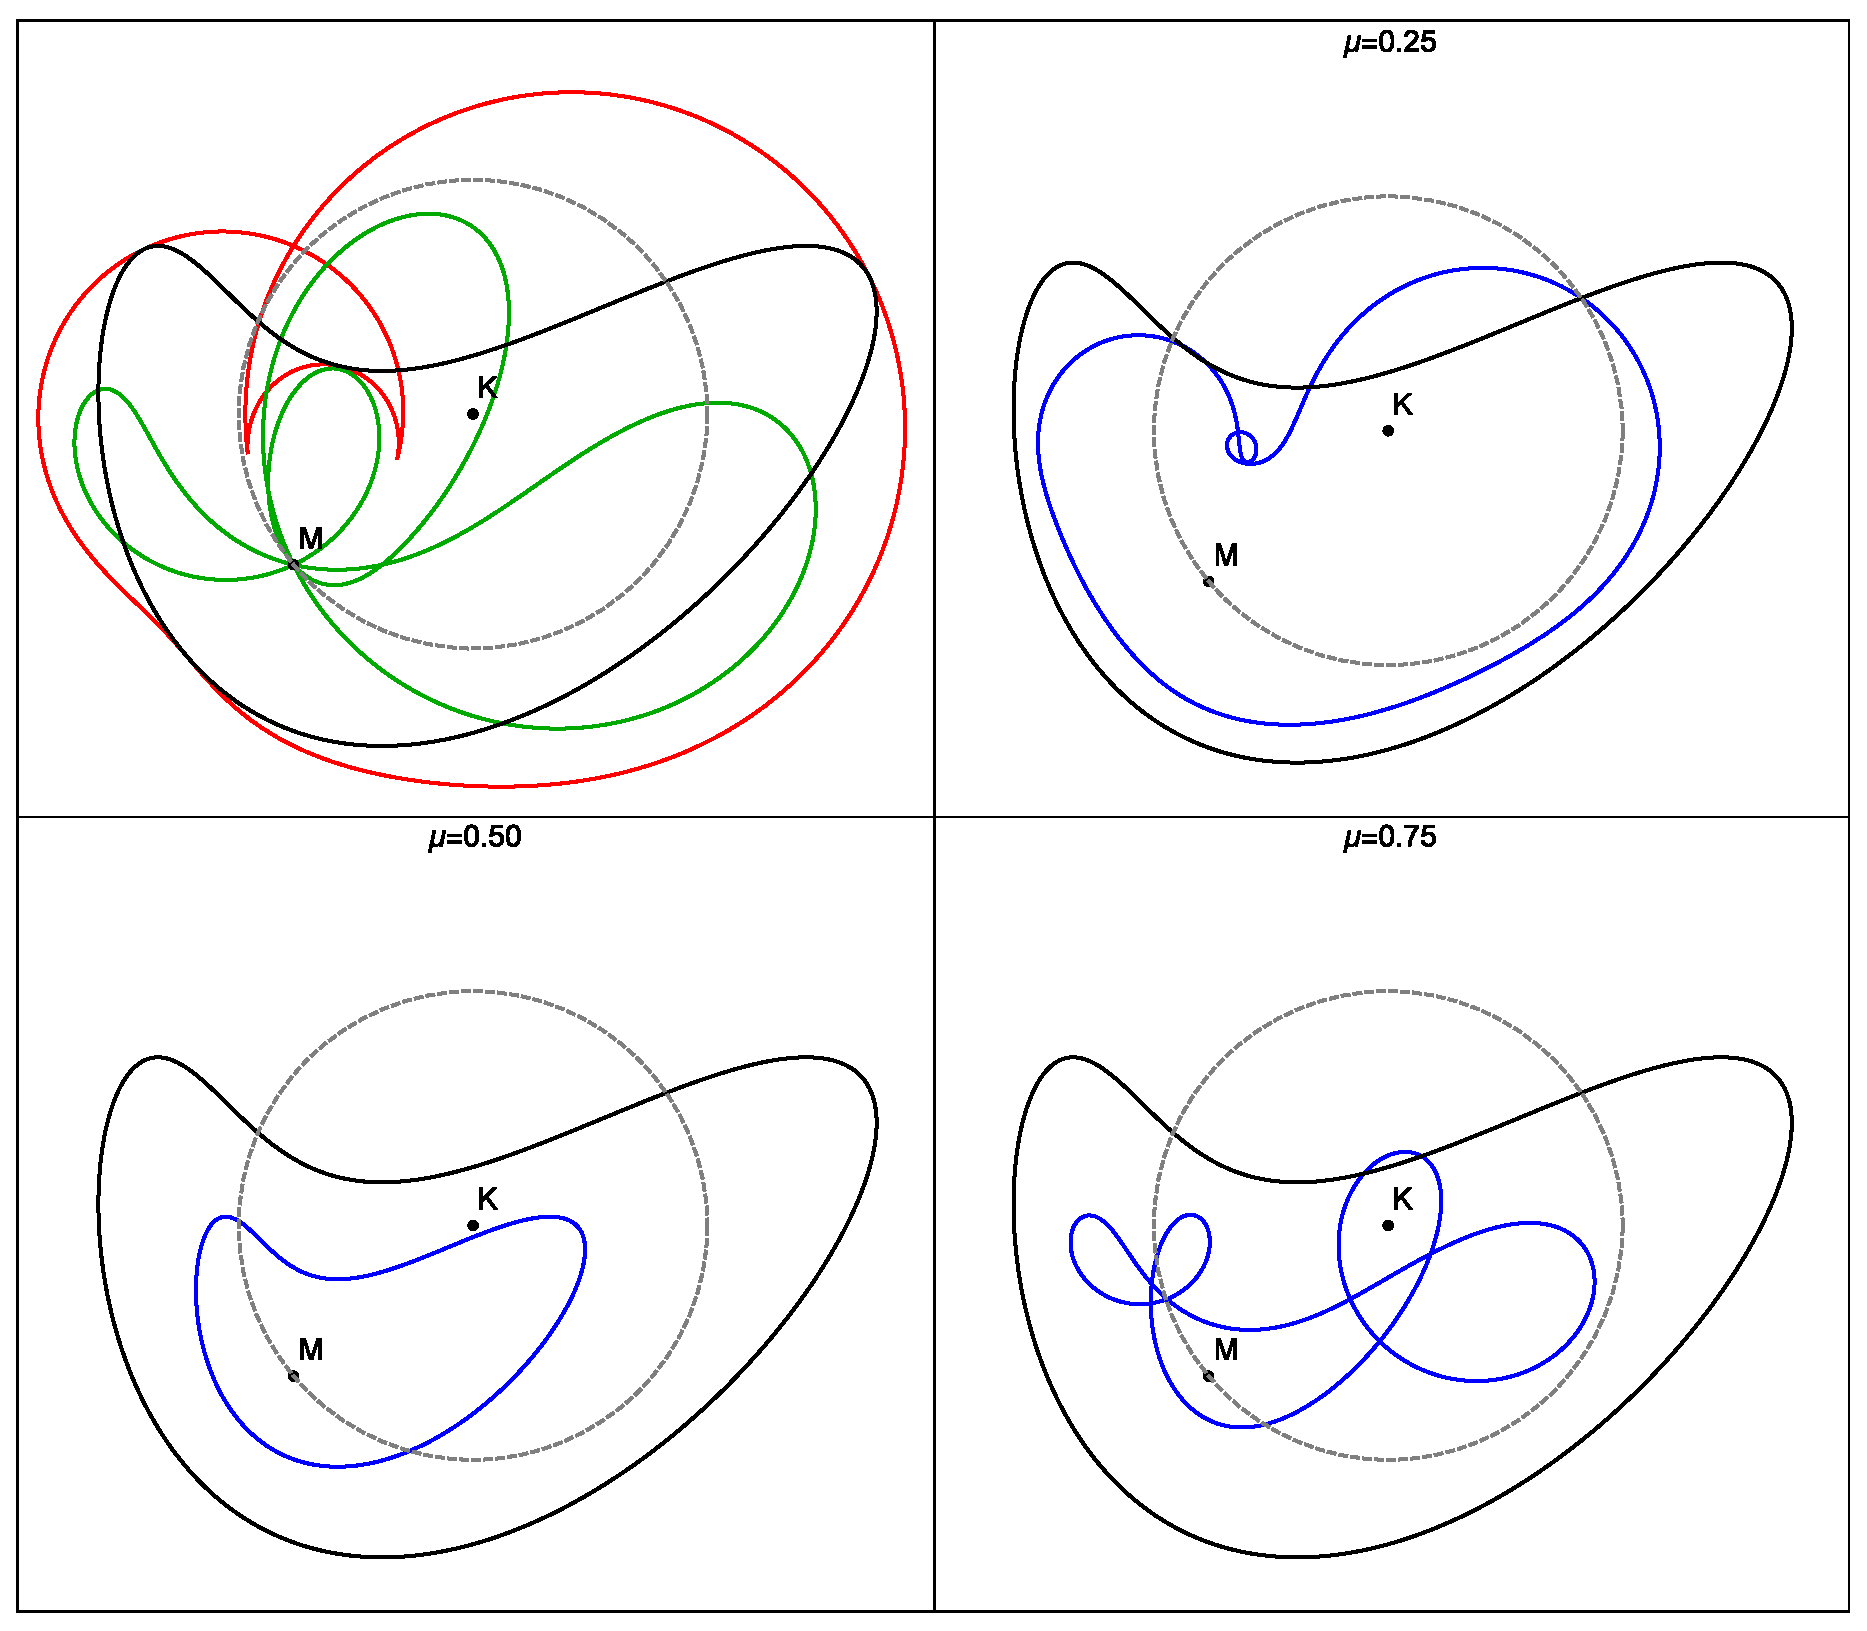
\includegraphics[width=\textwidth]{pics/0070_interpolated_concave.eps}
    \caption{\textbf{Top left}: a generic concave curve $\mathcal{C}$ (black) is shown as well as its curvature centroid $K$ and a circle about it where $M$ lies. Also shown are the pedal (red) and contrapedal (green) curves with respect to $M$. Note their areas are invariant for $M$ anywhere on a circle centered on $K$. \textbf{Top right, bottom left, bottom right}: the interpolated pedal curve (blue) for $\mu=0.25$, $0.5$, and $0.75$, respectively. Its area is also invariant for $M$ on a circle centered on $K$. Notice that at $\mu=0.5$ (bottom left) the interpolated pedal is homothetic (scale of 1/2) to $\mathcal{C}$ and its shape (and area) is independent of the location of $M$.}
    \label{fig:interp-concave}
\end{figure}